\section{Analysis and Case Study}
We used OMNeT++ as a simulation tool to explore the most
suitable model and algorithm for ThinkTogether. The study done by
Varga~\cite{A_OMNET_ESM01}
provides a brief introduction of OMNeT++, including Model Libraries, NED
language,
model structure. The paper also describes how to execute the simulation under a
powerful graphical user interface. Work done by Anggadjaja et
al.~\cite{EI_OMNET_ACT10}. features the
use of OMNeT++ based
simulation for a reliable point-to-point wireless transmission. The outcome could
provide inspiration for employing the P2P model in a wireless network. There
are several other papers~\cite{MM_OMNET_OMN08,XX_OMNET_ICQ12} explaining the
main infrastructure and
internal
design of OMNeT++.
%The team can gain overall understanding of the tool, through
%extensive papers above, and use OMNeT++ with efficiency and accuracy.

%Experimental data is the most scientific and objective way of verifying the
%efficiency of a particular network. There comes the simulation.
We evaluate several wireless and P2P frameworks~\cite{FBP_P2POVERLAY03},
such as MiXiM~\cite{XLL_MIXIM11}, OverSim~\cite{IBS_OVERSIM07}.
MiXiM is an OMNeT++ modeling framework created for mobile and fixed wireless
networks. MiXiM concentrates on the lower layers of the protocol stack, and offers
detailed models of radio wave propagation, interference estimation, radio transceiver
power consumption and wireless MAC protocols. OverSim is a flexible overlay network
simulation framework based on OMNeT++. OverSim includes several structured and
unstructured peer-to-peer protocols like Chord, Kademlia and Gia. Researchers can use
these protocols to run simulation for academic purpose as well as real world networks.

In our work, two network models will be built in order to observe the behavior
of data packets transferred in between the particular networks. One of the networking protocols
being used is Telnet, for which J. Postel et al~\cite{JJ_TEL83} provides the specification and
standards for using the protocol. This is a relatively old paper that was published in the early 1980s. The
paper draws a whole picture of the Telnet protocol from general consideration to
signal processing. Another protocol adopted is HTTP. There are wider
range of papers dedicated to HTTP. One of them is given by R Fielding~\cite{BJJH_HTTP1999}
, who provides a full-scaled overview, which can be used as a reference for modelling a network simulation.

%Multilayer Transmission

ThinkTogether is a communication application that contains multiple layers for
packet transmission. Data sent by each individual is handled differently. G.
Sekin et al~\cite{GF_COM00} provides an insight of how to manage multi
priority traffic in ATM network. The study is content-based video
objects. As the common characteristics shared between video stream and voice
stream, such as low tolerance in delay, jitter and packet. Unfortunately, there
is no evaluation involved in the paper, therefore the feasibility of the proposed
algorithm remains unknown.

After designing the model, we plan to create a working
network by creating a simulation using OMNeT++, as shown in Fig.~\ref{fig:sce}.
By creating this simulation we can have an idea of how the voice stream packets
are being transferred between the different nodes present in the network. Once
the simulation starts working for a basic scenario of just 2 leaf nodes, a
relayer and a cloud server, we will add more number of nodes to the simulation
and then analyse what changes are to be made to certain parameters of the
network so as to avoid any kind of latency and disturbance while transferring
the voice streams.

Presenters initialize services by sending voice packets to both relayers and
the cloud. Upon receiving the packets, the server stores them
locally and echoes back an acknowledgement. The services between presenter and
server is now finished. On the other side,
voice packets reach the relayer and will be directed to all attendees relayer
connects to, which is illustrated by \#6 and \#7 event in Fig.~\ref{fig:r_seq}.
Each attendees request the exact same voice data from the cloud.
Cloud handles the request by fetching corresponding data in server and sending
back the requested content. One can refer to events from \#11 to \#16 for
execution sequence details.



\section{Implementation: Data Distribution and Layers}

The simulation tests the efficiency in transferring voice data packets
with a fundamental model. This model lays the groundwork for future expansion,
and illustrates a simple way to consider a classroom scenario. The purpose of
the simulation is to investigate the feasibility, and more importantly, the efficiency of the
model. In the simulation, parameters such as packet drops, delay time, etc. are
collected and extracted to generate an output file for further analysis. The
output file is then used as
a foundation for performance analysis.


%In this paper our aim is to deploy a distributed the feature of voice
%streaming in the
%already developed application of Two Tall Totems called Think Together. In
%order to implement this feature we have
In our simulation of the model architecture, we use multiple nodes
as the leaf nodes in a network.
Then we also have some nodes that act as relayers in the network that will
transfer the voice stream from the presenter in the network to
the corresponding leaf nodes in the network. Along with all these nodes we also
have a cloud server which will act as a primary storage device for all the
voice streams that will be transmitted throughout the network. All the nodes will
have a direct link to the server so that if any of the leaf nodes (student
nodes in our scenario) want to retrieve any voice stream they can do so by
making a request to
the cloud server for that voice stream directly through the relayer (big node).

To simplify, we assume all the attendees are physically located in the same
classroom and they are subscribing to voice for the purpose of capturing the
information. This will eliminate potential influence caused by the difference
of
location, such as propagation delay. There are five components in the model:
presenter, relayer, cloud, server and attendee. Each component coordinates with
one another in order to offer recording services to attendees. There are two
test cases, one as a small-scaled network with two attendees, the other as a
slightly larger-scaled network with ten attendees. The simulation
is run in HTTP net,
masking the lower level network layers such as TCP and IP.


%Model Taxonomy

Figure~\ref{fig:sce} shows the overall picture of the simulation model in a
small-scaled case. It is broken done in four parts: sender (presenter), receiver (attendees),
mediator (relayers), and backup (cloud and server).

\begin{figure}[h!]
  \centering
    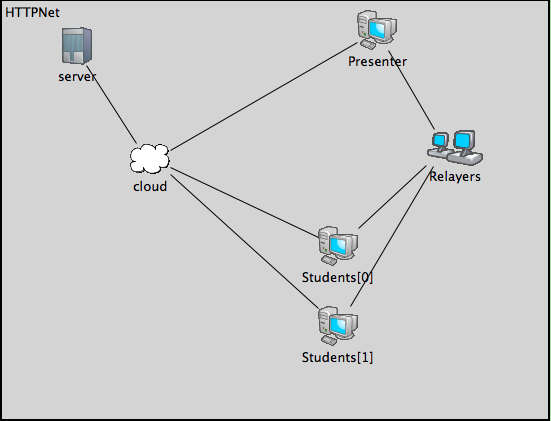
\includegraphics[width=0.5\textwidth]{figures/sce.png}
  \caption{Simulation in Omnet++}
  \label{fig:sce}
\end{figure}

Presenter is the starting point of the service. It does not rely on any outer
resource to trigger the sending process. Currently no packets other than
acknowledgement are sent to the presenters. In other words, one can view presenters
as a resource provider and there is no prerequisite for presenters to function.
There are two outgoing links connected to presenters. The one connected to
relayers is the main channel for delivering data. The one connected to cloud
transfers the same content, even though it is less demanding in terms of propagation
speed and processing time. A presenter sends voice packets to both links
simultaneously, and sets a timer for the next cycle.

The cloud server can be considered as a group in terms of services
purpose. They are both built to provide backup for attendees. There are two scenarios in
which attendees would need backup services. The first is when packets are lost by the
relayers and attendees will ask for complementary data from the cloud to ensure a
smooth stream. The second is when attendees are not able to attend
the class, but request a later review of that class. The server stores the
lectures in the format of voice stream and delivers it to attendees via cloud.
In this regard, the cloud is an interface between service providers and
receivers. In addition, once the network is scaled up to include multiple servers,
cloud acts as a coordinator that organizes the servers' actions.

The relayer acts as a router in this simple case simulation. Unlike servers,
the relayer
does
not store voice data, therefore all the attendees can not request data from the relayer
later on. It should be noted that this primary function is not yet implemented,
and will be
addressed later in the future model.

Attendees are students in the diagram. They receive voice packets from
presenters, regularly through relayers. It should be noted that attendees will
not send
acknowledgement back to presenters. When the network between relayers and
attendees are down, or for some reason, packets are lost in the regular
transmission routes, attendees will request the data from the server. The
target
users of the ThinkTogether application are attendees and presenters.
%Execution Sequence:

To collect data from multiple cycles, we set a timer for both presenter and
attendees based on an exponential distribution. After sending the voice
packets,
the presenter will create a timer that controls how long before the next cycle,
namely, the next time it starts sending the packets. The duration of the timer
is based on a exponential function, which allows random distribution in sending
packets. The same principle applies to the rate of sending request from attendees.
There is also a timer created by attendee that controls the rate of sending
requests to the cloud. In real life, an attendee will need the complementary data from cloud
only when the relayers fail to deliver it. However, in order to fully evaluate the
function, in the simulation we configure an attendee to request voice data from
the cloud whether the relayers go down or not.

\begin{figure}[h!]
  \centering
    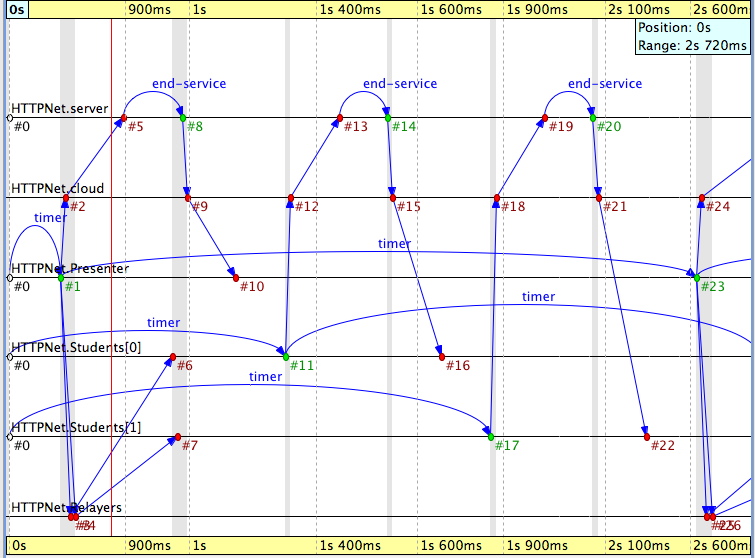
\includegraphics[width=0.5\textwidth]{figures/r_seq.png}
  \caption{Events in Time Sequence}
  \label{fig:r_seq}
  \vspace{-0.2in}
\end{figure}

The execution sequence is illustrated in Fig.~\ref{fig:r_seq}. It is a log file
generated by running small-scaled cases.

%\section{Deployment: Distributed Cloud}


